\chapter{Nauty algorithm}


In this section, we will present \Naut{} in detail. Our exposition is therefore largely inspired by McKay and Piperno's \emph{Practical Graph Isomorphism II}~\cite{mckay2014practical}, with the aim of providing a clearer and more accessible presentation.


\section{Introduction of the algorithm}
Nauty relies on the notion of a \hyperref[def:canonical form]{canonical form} to achieve its main objective: finding a canonical labelling of a graph and, consequently, determining its automorphism group. 

The canonical form allows us to bypass the intrinsic difficulty of the graph isomorphism problem. Instead of directly comparing two graphs, we associate each graph with a unique and standardised representative, called its canonical graph (or canonical form). Two graphs are then isomorphic if and only if their canonical forms are identical. In this way, an equivalence problem is transformed into an equality problem, which is significantly easier to handle computationally. For instance, when comparing a large collection of graphs, it is more efficient to compute the canonical form of each graph once and then compare these canonical forms, rather than perform an isomorphism test for every pair of graphs.


We begin by introducing the algorithm itself and describing the different functions that compose it, as well as the process used to compute the canonical form of a graph. We then examine the different pruning methods and explain how they can be used to construct the automorphism group.

\section{Search tree construction}

First of all, the algorithm itself is built upon a very specific type of graph: a \hyperref[def:graph]{tree}. More specifically, it relies on a search tree.

Informally, a search tree is a tree structure in which each node represents a state, and each branch corresponds to a specific action leading to another state. Since different actions produce different branches, the tree allows us to systematically explore all possible states starting from an initial state, with the goal of reaching a desired final state. In other words, we are performing a search over a tree structure, which explains the term \textit{search tree}.

However, its particularity is that the nodes of this tree correspond to sequences of vertices of a \hyperref[def: colouring]{coloured graph}. As we move down the tree, these sequences grow longer. These sequences define a colouring of the graph obtained by first assigning unique colours to the vertices in the sequence and then deducing, in a ``controlled'' manner, the colouring of the remaining vertices. The leaves of this tree correspond to sequences whose derived colouring is discrete. The root of this tree is therefore the empty sequence. 

To correctly construct this tree and find our canonical form, we will need several functions:

\begin{itemize}

  \item \textit{A refinement function}: Starting from a  partition, this function allows us to construct a new partition that is finer than the previous one.
  
  \item \textit{A target cell selection function}: Starting from a partition, this function allows us to choose a cell from this partition in order to create the ``children'' of the previous partition. 
  
  \item \textit{A node invariant function}: A function that allows us to efficiently compare the different nodes/leaves of our search tree in order to determine the canonical form of the graph.
  
\end{itemize}

\begin{figure}[ht]
  \centering
  \begin{tikzpicture}
\node[refbox] (refine0)
  {\textit{Refinement function}\\[2pt]
   {\footnotesize\normalfont refine the initial partition}};

\node[selbox, below=1.0cm of refine0] (select)
  {\textit{Target Cell selector function}\\[2pt]
   {\footnotesize\normalfont Select a cell to ``burst''}};

\node[refbox, below=1.0cm of select] (refine1)
  {\textit{Refinement function}\\[2pt]
   {\footnotesize\normalfont refine the new partition with respect to the selected cell}};

\node[invbox, below=1.0cm of refine1] (invar)
  {\textit{Node invariant function}\\[2pt]
   {\footnotesize\normalfont compute an invariant for the new partition}};

% arrows between pipeline boxes
\draw[mainarrow]
  (refine0) -- node[right, font=\scriptsize]{Initial partition/Root} (select);
\draw[mainarrow]
  (select)  -- node[right, font=\scriptsize]{New branch} (refine1);
\draw[mainarrow]
  (refine1) -- node[right, font=\scriptsize]{New node} (invar);


  \coordinate (loopright) at ($(current bounding box.east)+(1,0)$);
  \draw[looparrow]
    (invar.east) -|
    (loopright |- invar.east) --
    (loopright |- select.east) --
    (select.east);
  \node[font=\scriptsize, rotate=90, anchor=south, xshift=0.3cm]
    at ($(loopright |- invar.east)!0.5!(loopright |- select.east)$)
    {repeat for each node};

\end{tikzpicture}

  \caption{\textit{Search tree} construction in \Naut{}.}\label{fig:search-tree}
\end{figure}

These three functions are the fundamental components required to construct our search tree and find our canonical form. Before defining them formally, we will informally explain how they work and how they interact with each other to build our search tree.

Starting from a graph, we first apply the refinement function to obtain an \hyperref[def: colouring]{equitable partition}. This partition constitutes the root of our search tree.

Then, as long as we do not have a discrete partition, we apply the target cell selector to choose a cell from the current partition. Each branch represents a choice of element from the parent node's selected cell. This cell is then split into two cells using an individualisation method (which will be detailed later). For each branch, we apply the refinement function again to obtain a new partition, thereby creating a new node. Finally, on each node, we apply the node invariant function, which will be useful for determining the canonical form of our graph. We repeat this process until we obtain discrete partitions, which correspond to the leaves of our search tree. In summary, each node represents a partition, and each branch corresponds to the individualisation of a vertex from a chosen cell of the parent node.


However, there exist additional functions that are more specific to the implementation of the algorithm and that will be explained in the implementation section of this document.


\subsection{Formal definitions of the search tree functions}

Now that we have introduced the different functions composing our algorithm, we can formally define them and establish the properties of the associated search tree.

\vspace{0.4em}
\begin{definition}\label{def: refinement function}
  A \emph{refinement function} is a function
  \[
  R : \mathcal{G} \times \Pi \times V^* \to \Pi
  \]
  
  
  such that, for all  $G \mathrel{\in}\mathcal{G},  \pi\mathrel{\in}\Pi$ \ and  $\sigma\mathrel{\in}V^*$:
  
  \begin{enumerate}[label=\textit{R\arabic*.}]
    \item\label{RefinementRule:finer}
    $R (G, \pi, \sigma) \preccurlyeq\pi$.
    
    \item\label{RefinementRule:singleton}
     if $v \mathrel{\in}\sigma$\footnote{Here, the notation $v \in \sigma$ is used informally to indicate that the vertex $v$ appears in the sequence $\sigma$.}, then \{$v$\} is a cell of
    $R (G, \pi, \sigma)$.
    
    \item\label{RefinementRule:equivariance}
    for any $g \mathrel{\in} S_n$, we have
    $R (G^g, \pi^g, \sigma^g) = R {(G, \pi, \sigma)}^g$.
\end{enumerate}
\end{definition}

In other words, the refinement function returns a colouring that is finer than $\pi$, and any vertex belonging to the sequence $\sigma$ must form a singleton cell in the refined colouring. Furthermore, the function is equivariant under permutation: applying any $g \in S_n$ to the graph, the colouring, and the vertex sequence before or after the refinement yields the same result.

\vspace{0.5em}
\begin{definition}\label{def: target cell function}
  The \emph{target cell selector function} is a function  
  \[
  T : \mathcal{G} \times \Pi \times V^* \to 2^V
  \]
  
  such that, for all  $G \mathrel{\in}\mathcal{G},  \pi\mathrel{\in}\Pi$ \ and  $\sigma\mathrel{\in}V^*$:
  
  \begin{enumerate}[label=\textit{T\arabic*.}]
      \item if $R (G, \pi, \sigma)$ is discrete, then $T  (G, \pi, \sigma)$ = \cancel{0}.
      \item if $R (G, \pi, \sigma)$ is not discrete, then $T (G, \pi,\sigma)$ is a non-singleton cell of $R (G, \pi, \sigma)$.
     \item for any $g \mathrel{\in}S_n$, we have $T (G^g, \pi^g, \sigma^g) = T {(G, \pi, \sigma)}^g$.
  \end{enumerate}
  \end{definition}

  In other words, when the refinement function returns a discrete partition (corresponding to a leaf of the search tree) the target cell selector returns $\emptyset$. When the partition is non-discrete  (corresponding to an internal node) it returns a non-singleton cell of that partition. As with the refinement function, the target cell selector is equivariant under permutation: applying any $g \in S_n$ to the inputs before or after the selection yields the same result.

Now that all the formal definitions of the tree have been established, we can define the search tree $\mathcal{T} (G, \pi_0)$, which depends on an initial coloured graph $ (G, \pi_0)$. All the nodes of the tree are elements of $V^*$. This search tree has some characteristics to keep in mind:

\begin{itemize}
    \item The root of $\mathcal{T} (G, \pi_0)$ is the empty sequence ().
    \item if $\sigma$ is a node of $\mathcal{T} (G, \pi_0)$, let W = $T (G, \pi_0, \sigma)$. Then the children of $\pi$ are 
    \\ $\{\sigma\mathrel{\mid}\mathrel{\mid} w: w\mathrel{\in}W\}$.
    \item a node $\sigma$ of $\mathcal{T} (G, \pi_0)$ is a leaf iff $R (G, \pi_0, \sigma)$ is discrete.
    \item for any node $\sigma$ of $\mathcal{T} (G, \pi_0)$, define $\mathcal{T} (G, \pi_0, \sigma)$ to be the subtree of $\mathcal{T} (G, \pi_0)$ consisting of $\sigma$ and all its descendants.
    
\end{itemize}



To demonstrate the correctness of the algorithm, the pruning procedure that we will introduce, and to prove that we indeed obtain the canonical form of the graph, we need to establish several properties of this search tree.

\vspace{0.5em}

\begin{lemma}\label{lem: equivariance of the search tree}
  For any $G \mathrel{\in}\mathcal{G}, \pi_0\mathrel{\in}\Pi, g\mathrel{\in}S_n$ we have $\mathcal{T} (G^g, \pi_0^g) = \mathcal{T} {(G, \pi_0)}^g $.
  \end{lemma}

\vspace{-0.7em}
  \begin{proof}
    Let $\sigma = (\sigma_1, \ldots, \sigma_k)$ be a node of $\mathcal{T}(G, \pi_0)$, and let $\sigma^g = (\sigma_1^g, \ldots, \sigma_k^g)$ $\mathcal{T}(G^{g}, \pi_0^{g})$. We first show that $\mathcal{T}(G, \pi_0){^g} \subseteq \mathcal{T}(G^g, \pi_0^g)$.

    
    We proceed by induction on $s$, for $0 \leq s \leq k$, showing that ${[\sigma^g]}_s = (\sigma_1^g, \ldots, \sigma_s^g)$ is a node of  $\mathcal{T}(G^g, \pi_0^g)$.
    
    \textbf{Base case} ($s = 0$): The empty sequence $()$ is the root of any search tree.
    So ${[\sigma^g]}_0$ is trivially a node of $\mathcal{T}(G^g, \pi_0^g)$.
    
    \textbf{Inductive step}: Assume ${[\sigma^g]}_s = (\sigma_1^g, \ldots, \sigma_s^g)$ is a node of $\mathcal{T}(G^g, \pi_0^g)$. 
    
    Since $(\sigma_1, \ldots, \sigma_s, \sigma_{s+1})$ is a node of
    $\mathcal{T}(G, \pi_0)$, the element $\sigma_{s+1}$ was individualised to go from level $s$
    to level $s+1$. Since we apply $g$ to the entire structure, $\sigma_{s+1}$ is also mapped
    to $\sigma_{s+1}^g$, which is equivalent to directly individualising $\sigma_{s+1}^g$ in $G^g$
    with $\pi_0^g$. Hence ${[\sigma^g]}_{s+1} = (\sigma_1^g, \ldots, \sigma_s^g, \sigma_{s+1}^g)$ is a node of
    $\mathcal{T}(G^g, \pi_0^g)$.
    
    By induction, $\sigma^g$ is a node of $\mathcal{T}(G^g, \pi_0^g)$, hence
    $\mathcal{T}{(G, \pi_0)}^g \subseteq \mathcal{T}(G^g, \pi_0^g)$.
    
    The reverse inclusion follows by applying the same argument with $g^{-1}$
    in place of $g$, which gives
    $\mathcal{T}{(G^g, \pi_0^g)}^{g^{-1}} \subseteq \mathcal{T}(G, \pi_0)$,
    and therefore $\mathcal{T}(G^g, \pi_0^g) \subseteq \mathcal{T}{(G, \pi_0)}^g$.
    \end{proof}
  
  \begin{corollary}\label{cor: Corollary}
  Let $\sigma$ be a node of $\mathcal{T} (G,\pi_0)$ and let $g \mathrel{\in}\Aut (G, \pi_0)$. Then $\sigma^g$, is a node of $\mathcal{T} (G,\pi_0)$ and $\mathcal{T} (G, \pi_0, \sigma^g) = \mathcal{T} {(G, \pi_0, \sigma)}^g$.
  \end{corollary}

\vspace{-0.7em}
  \begin{proof}
    \leavevmode\\
    \textbf{Part 1} ($\sigma^g$ is a node of $\mathcal{T}(G, \pi_0)$):\\
    By \hyperref[lem: equivariance of the search tree]{Lemma 1}, we have: 
    \[
    \mathcal{T}(G^{g}, \pi_0^{g}) = \mathcal{T}{(G, \pi_0)}^{g}
    \]
    Since $g \in \Aut(G, \pi_0)$, we have $G^g = G$ and $\pi_0^g = \pi_0$, and therefore:
    \[
    \mathcal{T}(G, \pi_0) = \mathcal{T}{(G, \pi_0)}^{g}
    \]
    Since $\sigma$ is a node of $\mathcal{T}(G, \pi_0)$, $\sigma^g$ is a node of
    $\mathcal{T}{(G, \pi_0)}^g = \mathcal{T}(G, \pi_0)$.
    
    \textbf{Part 2} ($\mathcal{T}(G, \pi_0, \sigma^g) = \mathcal{T}{(G, \pi_0, \sigma)}^g$):\\
    We apply Lemma 1 to the subtree rooted at $\sigma$. Since $g$ maps each node
    of the subtree rooted at $\sigma$ to a node of the subtree rooted at $\sigma^g$,
    and since $g \in \Aut(G, \pi_0)$ implies $G^g = G$ and $\pi_0^g = \pi_0$,
    the same argument as in \hyperref[lem: equivariance of the search tree]{Lemma 1} gives both inclusions:
    \[\mathcal{T}{(G, \pi_0, \sigma)}^g \subseteq \mathcal{T}(G, \pi_0, \sigma^g)
    \quad \text{and} \quad
    \mathcal{T}(G, \pi_0, \sigma^g) \subseteq \mathcal{T}{(G, \pi_0, \sigma)}^g\]
    and therefore $\mathcal{T}(G, \pi_0, \sigma^g) = \mathcal{T}{(G, \pi_0, \sigma)}^g$.
    \end{proof}
  
  \begin{lemma}
      Let $\sigma$ be a node of $ (G,\pi_0)$ and let $\pi= R (G, \pi_0, \sigma)$. Then $\Aut(G,\pi$) is the   \hyperref[def:pointwise stabiliser]{point-wise stabiliser} of $\sigma$ in $\Aut(G,\pi_0)$.
  \end{lemma}



\vspace{-0.7em}
  \begin{proof}
    We show both inclusions to establish the equality.

    \textbf{Part 1} ($\Aut(G, \pi) \subseteq$ point-wise stabiliser of $\sigma$):\\
    Let $g \in \Aut(G, \pi)$. By \hyperref[RefinementRule:singleton]{R2}, for each $v \in \sigma$, $\{v\}$ is a singleton
    cell of $\pi = R(G, \pi_0, \sigma)$. Since $g$ is an automorphism of $(G, \pi)$, it must
    map each cell of $\pi$ to a cell of $\pi$. A singleton $\{v\}$ can only be mapped to
    itself, hence $v^g = v$ for every $v \in \sigma$, so $g$ stabilises $\sigma$ point-wise.
    
    \textbf{Part 2} (point-wise stabiliser of $\sigma$ $\subseteq \Aut(G, \pi)$):\\
    Let $g \in \Aut(G, \pi_0)$ be such that $g$ stabilises $\sigma$ point-wise, that is
    $\sigma^g = \sigma$. We want to show that $g \in \Aut(G, \pi)$ (so, $\pi^g = \pi$).
    By \hyperref[RefinementRule:equivariance]{R3} applied to $G$, $\pi_0$ and $\sigma$:
    \[R(G^g, \pi_0^g, \sigma^g) = R{(G, \pi_0, \sigma)}^g\]
    Since $g \in \Aut(G, \pi_0)$, we have $G^g = G$ and $\pi_0^g = \pi_0$, and since
    $g$ stabilises $\sigma$ point-wise, $\sigma^g = \sigma$. Therefore:
    \[  R(G, \pi_0, \sigma) = R{(G, \pi_0, \sigma)}^g\]
    which gives exactly $\pi = \pi^g$, and hence $g \in \Aut(G, \pi)$.
    \end{proof}


  Now that we have properly defined our search tree, we can discuss the node invariant function and how it allows us to compute the canonical form of the graph.


\vspace{0.5em} 
\begin{definition}\label{def: node variant}
  Let $\Omega$ be some totally ordered set. A \emph{Node invariant} is a function
  \[\phi : \mathcal{G} \times \Pi \times V^* \to \Omega\]

  Such that, for any $\pi_0 \mathrel{\in}\Pi$, $G \mathrel{\in}\mathcal{G}$ and distinct $\sigma, \sigma' \mathrel{\in}\mathcal{T} (G, \pi_0)$:


  \begin{enumerate}[label=\textit{$\phi$\arabic*.}]
      \item if $|\sigma| = |\sigma'|$ and $\phi(G,\pi_0, \sigma) < \phi(G,\pi_0, \sigma')$, then for every leaf $\sigma_1 \mathrel{\in}\mathcal{T} (G,\pi_0, \sigma)$ and leaf $\sigma_1' \mathrel{\in}\mathcal{T} (G,\pi_0, \sigma')$ we have $\phi(G,\pi_0, \sigma_1) < \phi(G,\pi_0, \sigma_2)$.
      \item if $\pi= R (G,\pi_0, \sigma)$ and $\pi' = R (G,\pi_0, \sigma')$ are discrete,\\
then $\phi(G,\pi_0, \sigma) = \phi(G,\pi_0, \sigma') \mathrel{\Leftrightarrow} G^\pi= G^{\pi'}$.
      \item for any $g \mathrel{\in}S_n$, we have $\phi(G^g,\pi_0^g, \sigma^g) = \phi(G,\pi_0, \sigma)$.
  \end{enumerate}
\end{definition}

{\sloppy
Property~1 ensures that the ordering induced by $\phi$ is consistent across the search tree: if two sequences of equal length satisfy $\phi(G,\pi_0,\sigma) < \phi(G,\pi_0,\sigma')$, then this strict inequality propagates to all descendant leaves, so no leaf below $\sigma$ can exceed any leaf below $\sigma'$. Property~2 states that at the leaves (where both refined partitions are discrete) the invariant captures the canonical labelling exactly: two leaves yield equal invariants if and only if they produce the same canonically labelled graph. Property~3 expresses that $\phi$ is invariant under permutation: applying any $g \in S_n$ to the graph, the colouring, and the vertex sequence before computing $\phi$ leaves the result unchanged.}

We can say that leaves $\sigma, \sigma'$ are \textit{equivalent} if  $\phi(G,\pi_0, \sigma) = \phi(G,\pi_0, \sigma')$. If this is the case, there is a unique $g \mathrel{\in}\Aut (G, \pi_0)$ such that $\sigma^g  = \sigma'$, with $g = R (G,\pi_0, \sigma') R {(G,\pi_0, \sigma)}^{-1}$. In other words, it connects equivalence of leaves to the automorphism group. We recall that $R(G, \pi_0, \sigma)$ is the discrete partition obtained by applying the refinement function along the sequence $\sigma$, and can therefore be viewed as a labelling of the vertices. Since both leaves are equivalent, their node invariants are equal, which means there exists a permutation $g$ such that:
\[R{(G, \pi_0, \sigma)}^g = R(G, \pi_0, \sigma')\]
Isolating $g$, we obtain:
\[g = R{(G, \pi_0, \sigma)}^{-1} \cdot R(G, \pi_0, \sigma')\]
If this permutation turns out to be an automorphism of $(G, \pi_0)$, it means that both leaves describe the same graph up to a relabelling of vertices, and are therefore equivalent.

By \hyperref[cor: Corollary]{Corollary 2}, if $\sigma$ is a leaf of $\mathcal{T}(G,\pi_0)$, then all leaves of the form $\sigma^g$,\\ where $g\in\Aut(G,\pi_0)$, are also leaves of $\mathcal{T}(G,\pi_0)$, and, due to the properties of $\phi$, they all share the same $\phi$-value, while no other leaf has this value. Consequently, for each leaf $\sigma$, we can say that:


\begin{align*}
\Aut(G,\pi_0) = \big\{R(G,\pi_0, \sigma')R{(G,\pi_0, \sigma)}^{-1} :\ &\sigma' \text{ is a leaf of } \mathcal{T}(G,\pi_0) \\
&\text{ with } \phi(G,\pi_0, \sigma') = \phi(G,\pi_0, \sigma)\big\}.
\end{align*}


This means that the automorphism group is generated entirely from leaves sharing the  same $\phi$-value as a fixed reference leaf $\sigma$: for each such leaf $\sigma'$, composing  the permutation $R(G,\pi_0,\sigma')$ with the inverse of $R(G,\pi_0,\sigma)$ yields an automorphism of $(G,\pi_0)$, and every automorphism arises this way. This holds for any choice of reference leaf $\sigma$.


We first define the \emph{canonical invariant} of $(G,\pi_0)$:
\[
\phi^*(G,\pi_0) \coloneqq \max\ \{\phi(G,\pi_0, \sigma): \sigma \text{ is a leaf of } \mathcal{T}(G,\pi_0)\}.
\]
Let $\sigma^*$ be any leaf of $\mathcal{T}(G, \pi_0)$ achieving this maximum. We can now define 
the \hyperref[def:canonical form]{canonical form} of $(G,\pi_0)$ as
\[
C(G, \pi_0) \coloneqq {(G, \pi_0)}^{R(G, \pi_0, \sigma^*)}.
\]
By the properties of $\phi$, $C(G, \pi_0)$ thus defined is independent of the choice of 
$\sigma^*$; in particular, any leaf achieving the maximum may be picked arbitrarily, and 
the resulting canonical form will always be the same.

In other words, the canonical invariant represents the maximum $\phi$-value achieved among 
all leaves of the search tree, and $\sigma^*$ is a leaf that achieves this maximum. The 
canonical form $C(G, \pi_0)$ is then obtained by applying the permutation associated with 
the leaf $\sigma^*$, namely $R(G, \pi_0, \sigma^*)$ (our canonical labelling), to the initial 
graph $(G, \pi_0)$. Here, we allow ourselves to use the refinement function itself to denote the permutation associated with the leaf $\sigma^*$. Indeed, since this leaf is discrete, it corresponds to an ordered partition of $V(G)$ into singletons (an ordering of the vertices); as the vertex set is already identified with $\{1,\ldots,n\}$, this ordering genuinely defines a permutation, and thus an element of $S_n$.
\subsection{Implementation strategies}

Now that we have all the theoretical tools in hand, we can begin discussing the implementation of the algorithm. Our implementation is based on the definitions of the algorithm, but it is not a direct or simplistic reproduction of its source code.

\newpage
\subsubsection{Implementation of the refinement function}


In order to ensure that the properties of the \hyperref[def: refinement function]{refinement function} defined in the search tree are respected, we must implement an algorithm that outputs a colouring that is equal to (or finer than) the original colouring. This motivates the need for an algorithm that computes a coarsest equitable colouring, in order to prevent refinement from being too aggressive and skipping intermediate structure in the search tree.

To construct our refinement function, we need two auxiliary functions: a function that refines a colouring so that it becomes an equitable colouring, and an individualisation function.

\vspace{0.5em}
\begin{definition}\label{def:refinement_algo}
  The function \emph{$F (G,\pi, \alpha)$} is our refinement algorithm (implemented in a label-invariant manner).
  
  \vspace{0.5em}
  \noindent\fbox{%
  \parbox{\linewidth- 2\fboxsep- 2\fboxrule}{%
  \textit{pseudo-code of $F(G,\pi, \alpha)$} (from~\cite{mckay2014practical})\label{algo:refinement}
  
  \vspace{0.5em}
  
  \begin{algorithmic}[1]
  \State\textbf{Data:} $\pi$ is the input colouring and $\alpha$ is a sequence of some cells of $\pi$
  \State\textbf{Result:} The final value of $\pi$ is the output colouring (equitable)
  
  \While{$\alpha$ is not empty \textbf{and} $\pi$ is not discrete}
      \State{Remove some element $W$ from $\alpha$}
      \For{each cell $X$ of $\pi$}
      \State\parbox[t]{0.9\linewidth}{Let $X_1, \ldots, X_k$ be the fragments of $X$ distinguished according to the number of edges from each vertex to $W$}
          \State{Replace $X$ by $X_1, \ldots, X_k$ in $\pi$}
          \If{$X \mathrel{\in}\alpha$}
              \State{Replace $X$ by $X_1, \ldots, X_k$ in $\alpha$}
          \Else\State{Add all but one of the largest of $X_1, \ldots, X_k$ to $\alpha$}
          \EndIf\EndFor\EndWhile\end{algorithmic}
  }%
  }
  \end{definition}


  This function is, at first glance, relatively straightforward to understand. However, it is important to carefully examine the different steps involved in the refinement process. We therefore describe these steps in more detail below.

  As stated in the pseudo-algorithm, we are given a graph $G$, a colouring $\pi$, and a sequence of cells of $\pi$ that will be used to refine the colouring. As long as not all cells in the sequence have been processed and the colouring is not yet discrete, we continue refining the colouring.
  
  At each iteration, we remove a cell $W$ from the sequence. Then, for every cell $X$ of the current colouring, we split $X$ into several cells $X_1, \ldots, X_k$ according to the number of edges each vertex of $X$ has with the vertices of $W$ (with respect to the graph $G$). We then replace the cell $X$ in the colouring by the newly created cells $X_1, \ldots, X_k$.
  
  If the cell $X$ already belongs to the sequence, we replace it in the sequence by the cells $X_1, \ldots, X_k$. Otherwise, we add all cells among $X_1, \ldots, X_k$ to the sequence except one, namely one of the largest cells. If several cells have the same maximum size, one of them is chosen arbitrarily and is not added to the sequence.

  \begin{figure}[ht]
    \centering
    \begin{tikzpicture}[
    every node/.style={font=\small},
    dot/.style={circle, fill=black, inner sep=2pt},
    bubble/.style={draw, ellipse, minimum width=2cm, minimum height=3cm, align=center},
    arrow/.style={->, thick, >=stealth}
  ]
  
  % Bubble W
  \node[bubble] (W) at (0, 0) {};
  \node[above=0.05cm] at (W.north) {$W$};
  \node[dot, label=left:$w_1$] (w1) at (0, 0.6) {};
  \node[dot, label=left:$w_2$] (w2) at (0, 0) {};
  \node[dot, label=left:$w_3$] (w3) at (0, -0.6) {};
  
  % Bubble X
  \node[bubble] (X) at (4, 0) {};
  \node[above=0.05cm] at (X.north) {$X$};
  \node[dot, label=right:$v_1$] (x1) at (4, 0.9) {};
  \node[dot, label=right:$v_2$] (x2) at (4, 0.3) {};
  \node[dot, label=right:$v_3$] (x3) at (4, -0.3) {};
  \node[dot, label=right:$v_4$] (x4) at (4, -0.9) {};
  
  % Edges
  \draw (x1) -- (w1);
  \draw (x2) -- (w1); \draw (x2) -- (w2);
  \draw (x3) -- (w1); \draw (x3) -- (w2);
  \draw (x4) -- (w1); \draw (x4) -- (w2); \draw (x4) -- (w3);
  
  % Arrow
  \draw[arrow] (5.5, 0) -- (7.0, 0) node[midway, above, font=\tiny] {fragment};
  
  % X1
  \node[bubble, minimum height=1.2cm] (X1) at (8.5, 2.6) {};
  \node[above=0.05cm] at (X1.north) {$X_1$};
  \node[dot, label=right:$v_1$] at (8.5, 2.6) {};
  \node[font=\tiny, right=0.1cm] at (X1.east) {1 edge to $W$};
  
  % X2
  \node[bubble, minimum height=1.5cm] (X2) at (8.5, 0.6) {};
  \node[above=0.05cm] at (X2.north) {$X_2$};
  \node[dot, label=right:$v_2$] at (8.5, 0.8) {};
  \node[dot, label=right:$v_3$] at (8.5, 0.4) {};
  \node[font=\tiny, right=0.1cm] at (X2.east) {2 edges to $W$};
  
  % X3
  \node[bubble, minimum height=1.2cm] (X3) at (8.5, -1.3) {};
  \node[above=0.01cm] at (X3.north) {$X_3$};
  \node[dot, label=right:$v_4$] at (8.5, -1.3) {};
  \node[font=\tiny, right=0.1cm] at (X3.east) {3 edges to $W$};
  
  \end{tikzpicture}
    \caption{Fragmentation of cell $X$ with respect to $W$.}\label{fig:refinement}
  \end{figure}


  \vspace{1em}

  \newpage
  
  \begin{definition}[Individualisation]\label{def:individualised_function}
    Let $\pi \in \Pi$ and let $v \in V$ be a vertex belonging to a non-singleton cell of $\pi$.
    The \emph{individualisation function}
    \[
    I : \Pi \times V \to \Pi
    \]
    maps $(\pi,v)$ to the partition $\pi' = I(\pi,v)$ defined, for every $w \in V$, by
    \[
    \pi'(w)=
    \begin{cases}
    \pi(w), & \text{if } \pi(w) < \pi(v) \text{ or } w=v, \\
    \pi(w)+1, & \text{otherwise}.
    \end{cases}
    \]
    The vertex $v$ is said to be \emph{individualised} in $\pi$.
    \end{definition}

  Intuitively, individualisation splits the cell containing $v$ into two parts: the vertex $v$ 
  itself becomes a singleton cell retaining the original position $\pi(v)$, while the remaining 
  vertices of that cell are shifted to position $\pi(v)+1$, immediately after $v$. Every cell 
  that originally preceded $v$'s cell is left unchanged, and every cell that came after is 
  shifted up by one position to make room; the relative order of the cells is thus preserved. Equivalently, $v$ is assigned a unique colour by removing it from its original cell and placing it into a new singleton cell, inserted immediately before the remaining vertices of that cell.


  
  Now we can define our refinement function. For a sequence of vertices $v_1, v_2, \ldots$, define
  \begin{itemize}
      \item $R(G, \pi_0, ()) = F(G, \pi_0, \text{ a list of all the cells of } \pi_0)$  
      \item $R(G, \pi_0, (v_1)) = F(G,\ I(R(G,\pi_0, ()), v_1),\ (\{v_1\}))$ 
      \item $R(G, \pi_0, (v_1, v_2)) = F(G,\ I(R(G,\pi_0, (v_1)), v_2),\ (\{v_2\}))$ 
      \item $R(G, \pi_0, (v_1, v_2, v_3)) = F(G,\ I(R(G,\pi_0, (v_1, v_2)), v_3),\ (\{v_3\}))$ 
      \item and so on, whose general form is, for $k \geq 1$:
    \end{itemize}
      \[
      R(G,\pi_0,(v_1,\ldots,v_{k-1}) \mid\mid v_k) = F\Big(G,\ I\big(R(G,\pi_0,(v_1,\ldots,v_{k-1})),\ v_k\big),\ (\{v_k\})\Big).
      \]

  \begin{proposition}\label{prop:refinement_properties}
    The refinement function $R$ defined above satisfies properties $\hyperref[RefinementRule:finer]{(R1)}-\hyperref[RefinementRule:equivariance]{(R3)}$.
  \end{proposition}
  
  \begin{proof}
    We prove each property separately.
  
    \textbf{Property \hyperref[RefinementRule:finer]{(R1)}}:
    By definition, the refinement function $R$ is obtained by repeatedly applying the individualisation operator $I$, with the refinement procedure $F$ applied on top of the partition produced by $I$. The operator $I$ only splits an existing cell into two cells, one of which is the singleton containing the individualised vertex, provided that the partition is not already discrete. Therefore, $I$ can only refine the current partition. The refinement function $F$ is designed to produce an equitable partition from the current partition. It can either split existing cells or leave them unchanged, but it never merges cells. Consequently, for every
    $G \in \mathcal{G}$, $\pi_0 \in \Pi$, and $\sigma \in V^*$, we have
    \[
      R(G,\pi_0,\sigma) \preccurlyeq \pi_0,
    \]
    and property \hyperref[RefinementRule:finer]{(R1)} holds.
  
    \textbf{Property \hyperref[RefinementRule:singleton]{(R2)}}:
    In the base case, no vertex is individualised, so the property is trivially
    satisfied for the empty sequence. For the subsequent steps, the operator
    $I$ creates a singleton cell containing the individualised vertex. Since $F$
    only refines the partition and never merges cells, this singleton remains
    unchanged after the refinement step. Therefore, every individualised vertex
    belongs to a singleton cell in the final partition, proving property
    \hyperref[RefinementRule:singleton]{(R2)}.
  
    \textbf{Property \hyperref[RefinementRule:equivariance]{(R3)}}:
    By definition of the individualisation operator, for any $g \in S_n$, we
    have
    \[
      I(\pi^g,v^g)=I(\pi,v){^g}.
    \]
    Indeed, the vertex $v$ belongs to the same cell in the transformed partition
    whether the permutation is applied before or after the individualisation
    step.
  
    Similarly, for the refinement function $F$, we have
    \[
      F(G^g,\pi^g,\alpha^g)=F(G,\pi,\alpha){^g}.
    \]
    The refinement procedure depends only on the structure of the graph and on
    the colouring of the vertices. In particular, the splitting of cells is
    determined by adjacency relations rather than by the labels of the vertices.
    Hence, applying $g$ before or after the refinement leads to equivalent partitions, which proves property
    \hyperref[RefinementRule:equivariance]{(R3)}.
  
    Therefore, the refinement function $R$ satisfies properties $\hyperref[RefinementRule:finer]{(R1)}-\hyperref[RefinementRule:equivariance]{(R3)}$.
  \end{proof}

In conclusion, the algorithm satisfies the required properties of a refinement function (as shown in \hyperref[prop:refinement_properties]{Proposition 4}) and performs well in practice. However, the refinement step is the most computationally expensive part of the algorithm, which is why special care must be taken in its implementation. Therefore, to reduce the overall running time, we will employ pruning techniques, which will be discussed later.


\subsubsection{Implementation of the target cell selector}

For the implementation of the \hyperref[def: target cell function]{target cell selector function} in the construction of the search tree, several strategies can be adopted. Choosing the right target cell at each step is important because it influences the shape and depth of the tree, and therefore the overall performance of the search.

In the original version of \Naut, McKay recommended selecting the first smallest non-singleton cell, as it increases the chance that the selected cell is part of an \hyperref[def:orbit]{orbit} of the group that stabilises the current sequence~\cite{mckay1981practical}. However, later studies showed that in certain cases, it is better to simply select the first non-singleton cell, regardless of its size~\cite{kirk1985efficiency}.

As a result, \Naut{} now supports two strategies for target cell selection that we can choose:

\begin{enumerate}
\item Always select the first smallest non-singleton cell.
\item Select the first cell that is joined in a non-trivial way to the largest number of other cells, where a non-trivial join means the number of edges between two cells is strictly between 0 and the maximum possible.
\end{enumerate}


In our implementation we will only use the first strategy. 

\vspace{0.5em}
\noindent\fbox{%
\parbox{\linewidth- 2\fboxsep- 2\fboxrule}{%
\textit{pseudo-code of targetCellSelector}

\vspace{0.5em}

\begin{algorithmic}[1]
\State\textbf{Data:} a partition $\pi = (X_1, \ldots, X_k)$
\State\textbf{Result:} the first non-singleton cell of minimum size in $\pi$
\State\Return{the first $X \in \pi$ such that $|X| > 1$ and
$|X| = \min_{Y \in \pi,\ |Y| > 1} |Y|$}
\end{algorithmic}
}%
}


\subsubsection{Intermediate search tree construction}

All the functions required to define the search tree have now been implemented. The following example illustrates the construction of the search tree for the graph $K_{1,3}$ using target-cell selection and equitable refinement. In the tree, individualised vertices are represented by double circles and the encircled set in each partition denotes the current target cell.

\vspace{2em}

\begin{figure}[htbp]
  \centering
  \resizebox{\linewidth}{!}{%
  
% Encircle a target cell inline.
\newcommand{\tc}[1]{%
\tikz[baseline= (c.base)]{
\node[
    draw,
    ellipse,
    inner sep=1.5pt,
    outer sep=0pt,
    line width=0.4pt
] (c) {#1};
}%
}


\newcommand{\ktgraph}[3]{%
\begin{tikzpicture}[
    scale=0.42,
    every node/.style={
        circle,
        draw,
        inner sep=0pt,
        minimum size=6mm,
        font=\tiny,
        line width=0.5pt
    }
]

\node (g0) at (0,0) {0};

\node[#1] (g1) at (-1.15,1.15) {1};
\node[#2] (g2) at (0,1.55) {2};
\node[#3] (g3) at (1.15,1.15) {3};

\draw (g0)--(g1);
\draw (g0)--(g2);
\draw (g0)--(g3);

\end{tikzpicture}%
}






\begin{tikzpicture}[
    every node/.style={font=\small}
]


% ---------- Initial partition ----------
\node[anchor=north,align=center] (init) at (8.75,14)
{
\ktgraph{}{}{}\\[2pt]
$[\,0,1,2,3\,]$
};


% ---------- First refinement ----------
\node[anchor=north,align=center] (root) at (8.75,10)
{
\ktgraph{}{}{}\\[2pt]
$[\,0 \mid \tc{1,2,3}\,]$
};

\draw[
->,
line width=0.5pt
]
(init.south) --
(root.north)
node[midway,right]
{\scriptsize First Refinement};


% ---------- Level 1 ----------
\node[anchor=north,align=center] (A) at (1.75,6)
{
\ktgraph{double}{}{}\\[2pt]
$[\,0 \mid 1 \mid \tc{2,3}\,]$
};

\node[anchor=north,align=center] (B) at (8.75,6)
{
\ktgraph{}{double}{}\\[2pt]
$[\,0 \mid 2 \mid \tc{1,3}\,]$
};

\node[anchor=north,align=center] (C) at (15.75,6)
{
\ktgraph{}{}{double}\\[2pt]
$[\,0 \mid 3 \mid \tc{1,2}\,]$
};


% ---------- Leaves ----------
\node[anchor=north,align=center] (L1) at (0,1.2)
{
\ktgraph{double}{double}{}\\[2pt]
$[\,0 \mid 1 \mid 2 \mid 3\,]$
};

\node[anchor=north,align=center] (L2) at (3.5,1.2)
{
\ktgraph{double}{}{double}\\[2pt]
$[\,0 \mid 1 \mid 3 \mid 2\,]$
};

\node[anchor=north,align=center] (L3) at (7,1.2)
{
\ktgraph{}{double}{ }\\[2pt]
$[\,0 \mid 2 \mid 1 \mid 3\,]$
};

\node[anchor=north,align=center] (L4) at (10.5,1.2)
{
\ktgraph{}{double}{double}\\[2pt]
$[\,0 \mid 2 \mid 3 \mid 1\,]$
};

\node[anchor=north,align=center] (L5) at (14,1.2)
{
\ktgraph{}{}{double}\\[2pt]
$[\,0 \mid 3 \mid 1 \mid 2\,]$
};

\node[anchor=north,align=center] (L6) at (17.5,1.2)
{
\ktgraph{}{double}{double}\\[2pt]
$[\,0 \mid 3 \mid 2 \mid 1\,]$
};


% ---------- Target cell labels ----------
\draw[dashed,->]
(root.east) -- ++(1.2,0)
node[right]{\scriptsize Target cell};

\draw[dashed,->]
(A.east) -- ++(1.1,0)
node[right]{\scriptsize Target cell};

\draw[dashed,->]
(B.east) -- ++(1.1,0)
node[right]{\scriptsize Target cell};

\draw[dashed,->]
(C.east) -- ++(1.1,0)
node[right]{\scriptsize Target cell};


% ---------- Edges ----------
\draw (root.south) -- (A.north)
node[midway,above left] {$1$};

\draw (root.south) -- (B.north)
node[midway,right] {$2$};

\draw (root.south) -- (C.north)
node[midway,above right] {$3$};


\draw (A.south) -- (L1.north)
node[midway,left] {$2$};

\draw (A.south) -- (L2.north)
node[midway,right] {$3$};


\draw (B.south) -- (L3.north)
node[midway,left] {$1$};

\draw (B.south) -- (L4.north)
node[midway,right] {$3$};


\draw (C.south) -- (L5.north)
node[midway,left] {$1$};

\draw (C.south) -- (L6.north)
node[midway,right] {$2$};


\end{tikzpicture}


  }
  
\caption{Search tree for $K_{1,3}$.}\label{fig:nauty-tree-k13}

\end{figure}


\subsubsection{Implementation of the node invariant}

Once the search tree construction is in place, the next step is to define the \hyperref[def: node variant]{node invariant function}, which will allow us to determine the canonical form. To compute this function, we can rely on two related sources:

\begin{enumerate}
  \item For each node $\sigma$, there is a colouring $R(G,\pi_0, \sigma)$. We can use its properties to extract the number and size of the cells, as well as combinatorial properties of the coloured graph.
  \item We can use intermediate states of the refinement algorithm as a node is processed, such as the position and size of the cells produced during the refinement procedure, and various edge counts determined during the computation. If $f(\sigma)$ is a function of this information (computed during the calculation of $R(G,\pi_0, \sigma)$ and from the resulting coloured graph) then the vector $(f([\sigma]_0), f([\sigma]_1), \ldots, f(\sigma))$, with lexicographic ordering, satisfies the characteristics required for a node invariant. In \Naut, the value of $f(\sigma)$ is an integer.
\end{enumerate}

Another potential method is based on the concept of the \textit{quotient graph}\footnote{Informally, the \emph{quotient graph} $Q(G,\pi)$ of a coloured graph $(G,\pi)$ is the graph whose vertices are the cells of $\pi$. Two cells $X_i$ and $X_j$ are joined by an edge whenever some vertex in $X_i$ is adjacent (in $G$) to some vertex in $X_j$. The quotient graph may also contain self-loops when $i=j$.} $Q(G,\pi)$, assuming that the colouring $\pi$ of graph $G$ is equitable. All vertices of $Q(G,\pi)$ are cells of $\pi$, and they include information about the size and number of the cell. For any two cells $C_1, C_2 \mathrel{\in}\pi$, possibly equal, the corresponding vertices in $Q(G,\pi)$ are connected by an edge labelled with the number of edges in $G$ between $C_1$ and $C_2$.

The node invariant computed by \Naut{} is a deterministic function of the sequence of quotient graphs $Q(G, R(G, \pi_0, [\sigma]_i))$ for $i = 0, \ldots, |\sigma|$. Therefore, one could in principle use the sequence of quotient graphs directly to construct the node invariant, but doing so would be too costly in both time and memory.

In our implementation, we rely on the first source described above: the number and size of the cells, together with combinatorial properties of the coloured graph, form the basis of our node invariant. Several invariant methods have been implemented in order to compare their efficiency and computational speed. Some of these methods were taken from the \Naut{} user guide~\cite{mckay2024nug}, where they are described as \textit{vertex invariants} in Brendan D. McKay's implementation; these methods were originally intended to assist the refinement function by promoting further cell splitting. We do not elaborate on this refinement-assisting role here, as our implementation follows the traditional structure of the algorithm, in which cell splitting is handled solely by the refinement procedure. Since these vertex invariants are deterministic functions of combinatorial properties of the coloured graph, we repurposed them as node invariants rather than as refinement aids.

Since this function is called at each node creation, it is important that its computation remains fast in order to avoid slowing down the algorithm. The following sections detail each of these methods, along with a brief discussion of their computational complexity and how they compare to one another.

Here is the exhaustive list of invariant methods that we have implemented so far:

\begin{enumerate}
  \item \textit{triangle per cell}: for each cell of the partition, we compute the number of triangles contained in that cell. This yields a vector whose $i$-th entry is the number of triangles contained in the $i$-th cell of the partition. This vector constitutes the node invariant. During the search, node invariants are then compared lexicographically to determine the best invariant encountered so far.
  
  \vspace{0.5em}
  \noindent\fbox{%
    \parbox{\linewidth- 2\fboxsep- 2\fboxrule}{%
    \textit{Pseudo-code of InvariantTrianglePerCell}
  
    \vspace{0.5em}
  
    \begin{algorithmic}[1]\label{algo:invariant_triangle_by_cell}
    \State\textbf{Data:} A graph $G$, a cell $C = \{v_1, \ldots, v_k\}$
    \State\hspace{1.5em} $N(u)$ denotes the ordered neighbour list of $u$ in $G$
    \State\textbf{Result:} The number of triangles contained in $C$
  
    \vspace{0.5em}
  
    \State$\mathit{count} \gets 0$
    \For{each $u \in C$}
        \For{each $v \in N(u) \cap C$ such that $v > u$}
            \For{each $w \in N(u) \cap N(v) \cap C$ such that $w > v$}
                \State$\mathit{count} \gets \mathit{count} + 1$
            \EndFor\EndFor\EndFor\State\Return$\mathit{count}$
    \end{algorithmic}
    }%
  }

  For counting the number of triangles in a cell, the most classical approach enumerates all triplets of vertices $(u, v, w)$ from the cell and checks for each one whether all three edges exist, running in $O(n^3)$ where $n$ is the number of vertices in the cell. A faster approach exploits the sorted neighbour lists $N(v)$: for each vertex $u \in C$, one iterates over its neighbours $v$ in the cell with $v > u$, then looks for common neighbours $w$ of both $u$ and $v$ still in the cell with $w > v$. Since the neighbour lists are sorted, each such lookup runs in $O(d)$ where $d$ is the largest number of neighbours that any vertex in the cell has, yielding an overall complexity of $O(n \cdot d^2)$. 

  \item\textit{two paths by cell}: for each cell of the partition, we examine every walk of length two starting from a vertex of that cell, and weight each such walk by the cell it reaches (which may be the starting vertex itself). Here, each cell of the partition is represented by an integer, namely its index within the partition, denoted $\mathrm{cellIndex}(v)$ in the code. The invariant of a cell $C$ is then obtained by summing, over every vertex $v \in C$ and every vertex $w$ reachable from $v$ by a walk of length two, the index of the cell containing $w$. This yields a single integer representing the invariant of the cell. This method is a \textit{vertex invariant} taken from the \Naut{} user guide, which we have therefore repurposed as a node invariant~\cite{mckay2024nug}; since only its high-level description was available to us, rather than the corresponding source code, it had to be reconstructed and generalised to fit our cell-based framework.
  

\vspace{0.5em}
\noindent\fbox{%
\parbox{\linewidth- 2\fboxsep- 2\fboxrule}{%
\textit{pseudo-code of InvariantTwoPathsByCell}

\vspace{0.5em}

\begin{algorithmic}[1]\label{algo:invariant_two_paths_by_cell}
    \State\textbf{Data:} A graph $G$, a cell $C = \{v_1, \ldots, v_k\}$
  \State\textbf{Result:} the invariant value of the cell $C$
  \State$\mathit{count} \gets 0$

  \ForAll{vertices $v \in C$}
      \ForAll{neighbours $u \in N(v)$}
          \State$\mathit{count} \gets \mathit{count} + \sum_{w \in N(u)} \mathrm{cellIndex}(w)$
      \EndFor{}
  \EndFor{}

  \State\Return{$\mathit{count}$}
  \end{algorithmic}
}%
}

The computation of this invariant is divided into two steps. First, for every vertex $u \in V$, we precompute the value $S(u)=\sum_{w \in N(u)} \mathrm{cellIndex}(w)$ by scanning the adjacency list of each vertex once. Since every edge is traversed at most twice, this preprocessing step requires $O(n+m)$ time, where $n$ is the number of vertices and $m$ is the number of edges. Once these values have been computed, the invariant of a cell $C$ is obtained by iterating over every vertex of the cell and summing the precomputed values of its neighbours. The running time for one cell is therefore $O\!\left(\sum_{v\in C}\deg(v)\right)$. Since the cells form a partition of the vertex set, each vertex is processed exactly once when computing the invariant for all cells, yielding an overall running time of $O(n+m)$.

\item\textit{triple by cell}: this method is also a \textit{vertex invariant} taken from the \Naut{} user guide, which we have likewise repurposed as a node invariant~\cite{mckay2024nug}. However, since no source code was available, we had to reconstruct the method from its description. The idea is to consider, for each cell, every triple ofvertices $\{u,v,w\}$ it contains. For each triple, we count the number of vertices $x$ of the graph that are adjacent to an odd number of the vertices of $\{u,v,w\}$ (that is, adjacent to exactly one or exactly three of them); this count is the weight of the triple, and it is added
to the counter of each of the three vertices $u$, $v$ and $w$. The final invariant of the cell
is the sum of these counters over every vertex it contains. The main drawback of this method
is that it is computationally expensive, as it requires enumerating every triple of vertices
in each cell, which can be prohibitive for large cells.

\vspace{0.5em}
\noindent\fbox{%
\parbox{\linewidth- 2\fboxsep- 2\fboxrule}{%
\textit{pseudo-code of InvariantTripleByCell}

\begin{algorithmic}[1]\label{algo:invariant_cell_triples_by_cell}
    \State\textbf{Data:} A graph $G$, a partition $\pi = (C_1,\ldots,C_k)$
    \State\textbf{Result:} the invariant value of each cell of $\pi$
    
    \State$I \gets (0,\ldots,0)$ of size $k$
    
    \ForAll{cells $C_i \in \pi$}
        \ForAll{triples of vertices $\{u,v,w\} \subseteq C_i$}
            \State$weight \gets 0$
            
            \ForAll{vertices $x \in V(G)$}
                \If{$|N(x)\cap\{u,v,w\}|$ is odd}
                    \State$weight \gets weight + 1$
                \EndIf{}
            \EndFor{}
            
            \State$I[i] \gets I[i] + weight$
        \EndFor{}
    \EndFor{}
    
    \State\Return{$I$}
\end{algorithmic}
}%
}

For a cell $C_i$ of size $|C_i|$, the number of triples $\{u,v,w\} \subseteq C_i$ is $\binom{|C_i|}{3} = O(|C_i|^3)$, and computing the weight of a single triple requires
scanning all $n$ vertices of $G$. Evaluating the invariant on $C_i$ therefore costs
$O(|C_i|^3 \cdot n)$. Since this is computed for every cell of $\pi$, and $\sum_i |C_i| = n$, the worst case gives an overall cost of $O(n^4)$. In practice, cells are usually much smaller once the standard refinement has run, keeping the actual cost far below this bound.
\end{enumerate}



\subsection{Pruning strategies}

To avoid generating unnecessary information in our search tree,which would result in an overly large tree, we aim to construct the most optimised tree possible. To achieve this, we can apply \textit{pruning} techniques to the tree: eliminating redundant branches so that only a fraction of the original tree needs to be generated. We can define two types of pruning strategies to optimise our construction:

$\mathcal{P}_A(\sigma, \sigma')$: We remove $T(G, \pi_0, \sigma')$ whenever $\sigma, \sigma'$ are distinct nodes of $T(G, \pi_0)$ satisfying $|\sigma| = |\sigma'|$ and $\phi(G,\pi_0,\sigma) > \phi(G,\pi_0,\sigma')$.

$\mathcal{P}_B(\sigma, \sigma')$: We remove $T(G, \pi_0, \sigma')$ whenever $\sigma, \sigma'$ are distinct nodes of $T(G, \pi_0)$ satisfying $|\sigma| = |\sigma'|$ and $\phi(G,\pi_0,\sigma) \neq \phi(G,\pi_0,\sigma')$.

$\mathcal{P}_C(\sigma, g)$: We remove $T(G, \pi_0, \sigma')$ whenever $g \in \Aut(G,\pi_0)$ and $\sigma < \sigma'$ are nodes of $T(G, \pi_0)$ such that $\sigma^g = \sigma'$.

Informally, each pruning method serves a distinct purpose. The method $\mathcal{P}_A$ discards branches whose invariant cannot reach the maximal value: at each level of the tree, we keep track of the best invariant found so far, and any other node at the same level with a strictly worse invariant has its branch pruned. The method $\mathcal{P}_B$ is somewhat more subtle. Rather than comparing the current node to the best node found so far, it is compared to a reference node, taken as the node at the same level lying on the first path leading to the first leaf. If the two invariants differ, the current subtree is pruned. Here, the goal is not really to find the best invariant, but rather to uncover new automorphisms. Combining the two methods, a branch is pruned only when both $\mathcal{P}_A$'s and $\mathcal{P}_B$'s conditions are satisfied. 
In other words, the current node is pruned if its invariant is strictly 
worse than the best invariant found so far and if it differs from the 
invariant of the reference node. Finally, the method $\mathcal{P}_C$ exploits automorphisms already discovered during the search. Suppose an automorphism $g \in \Aut(G,\pi_0)$ maps the current node $\sigma$ to another node $\sigma^g$ that has already been explored. Since the corresponding subtrees are isomorphic, exploring both would be redundant; the subtree rooted at $\sigma^g$ can therefore be discarded.


Despite these pruning strategies, we must ensure that our search tree, along with the node invariant function, remains functionally correct. To this end, we require a theorem that guarantees the validity of the overall construction.

\vspace{0.4em}

\begin{theorem}\label{Theo: prunning}
    Consider any $G \mathrel{\in}\mathcal{G}$ and $\pi_0 \mathrel{\in}\Pi$
    \begin{itemize}
    \item Suppose any sequence of operations of the form $\mathcal{P}_A (\sigma, \sigma')$ or $\mathcal{P}_C (\sigma, g)$ are performed. \\ Then there remains at least one leaf $\sigma_1$ with $\phi(G,\pi_0, \sigma_1) = \phi^* (G,\pi_0)$.
    \item Let $\sigma_0$ be some fixed leaf of $T (G, \pi_0)$. Suppose any sequence of operations of the form $\mathcal{P}_B (\sigma, \sigma')$ $\mathcal{P}_C (\sigma'', g)$ are performed, where $\phi(G,\pi_0, \sigma'') \neq\phi(G,\pi_0, {[\sigma_0]}_{|\sigma''|})$. Let $g_1, \ldots, g_k$ be the automorphisms
used in the operations $\mathcal{P}_C$ that were performed, and let $A = \{g \mathrel{\in}\Aut(G,\pi_0)$: $\sigma_0^g$ is a remaining leaf\}. Then $\Aut(G,\pi_0)$ is generated by $\{g_1, \ldots, g_k\} \,\cup\, A$.
\end{itemize}
\end{theorem}


\begin{proof}
  To prove the first point, let $\sigma_1$ denote the lexicographically smallest leaf satisfying $\phi(G,\pi_0,v_1)=\phi^*(G,\pi_0)$.
  Operation $\mathcal{P}_A$ only removes branches whose invariant cannot reach the maximal value, while operation $\mathcal{P}_C$ always preserves the lexicographically smallest representative of an automorphism class. Consequently, $\sigma_1$ cannot be removed. Therefore, at least one leaf with maximal invariant always remains after any sequence of pruning operations.
  
  For the second point, let $g\in\mathrm{Aut}(G,\pi_0)$ and consider the corresponding leaf $\sigma_0^g$.
  
  If $\sigma_0^g$ is still present after pruning, then by definition $g\in A$.
  
  Otherwise, $\sigma_0^g$ must have been removed by an operation $\mathcal{P}_C(\sigma'',g_i)$. It cannot be removed by $\mathcal{P}_B(\sigma', \sigma)$ because it only removes leaves inequivalent to $\sigma_0$. This implies that there exists a lexicographically smaller equivalent leaf, namely
  \[
  \sigma_0^{gg_i^{-1}}<\sigma_0^g.
  \]
  
  If this new leaf has also been removed, the same reasoning applies. Repeating this process produces a strictly decreasing sequence of equivalent leaves
  \[
  \sigma_0^g >
  \sigma_0^{gg_i^{-1}} >
  \sigma_0^{gg_i^{-1}g_j^{-1}} >
  \cdots
  \]
  
  Since the lexicographic order on the finite set of leaves is well-founded, this sequence must eventually terminate at a remaining leaf. Hence, there exists $h\in\langle g_1,\ldots,g_k\rangle$
  such that $\sigma_0^{gh}$ is a remaining leaf. By definition of $A$, we have $gh\in A$, and therefore $ g=(gh)h^{-1}$ where $gh\in A$ and $h^{-1}\in\langle g_1,\ldots,g_k\rangle$.
  
  Since $g$ was arbitrary, every automorphism belongs to the group generated by
  \[
  \{g_1,\ldots,g_k\}\cup A,
  \]
  which proves the result.
  \end{proof}

Informally, this theorem and its proof establish that pruning can never eliminate every leaf realising the maximal invariant: at least one such leaf always survives. The second part of the theorem further shows that the full automorphism group $\Aut(G,\pi_0)$ remains recoverable despite pruning: it is generated by the witnesses $g_1,\ldots,g_k$ collected along the $\mathcal{P}_C$ operations, together with the automorphisms in $A$ corresponding to the surviving leaves in the orbit of a fixed reference leaf $\sigma_0$. In other words, even though the vast majority of leaves equivalent to $\sigma_0$ are discarded during the search, the automorphisms they correspond to are never lost: each one can be recovered as a composition of an element of $A$ and an element of the subgroup generated by $g_1,\ldots,g_k$.

The $\mathcal{P}_A$ pruning strategy is relatively straightforward to implement. At each level of the search tree, we simply compare the node invariant of the node currently being explored with the best node invariant encountered so far at the same level. If the invariant of the current node is smaller than the best one found previously, then the corresponding subtree can safely be discarded.

The $\mathcal{P}_B$ strategy is slightly more involved. Instead of comparing the current node with the best node encountered so far, we compare its node invariant with that of a reference node. This reference node is chosen as the node at the same level lying on the first path leading to the first leaf. If the two node invariants differ, the current subtree is pruned. Conversely, branches whose node invariants coincide with those of the reference path remain candidates for discovering new automorphisms.

Finally, the $\mathcal{P}_C$ strategy exploits the automorphisms that have already been discovered during the search. Suppose that an automorphism $g \in \Aut(G,\pi_0)$ maps the current node $\sigma$ to another node $\sigma^g$ that has already been explored. Since the corresponding subtrees are isomorphic, exploring both of them would be redundant. Consequently, the subtree rooted at $\sigma^g$ can be discarded.

Implementing this strategy is considerably more challenging than implementing $\mathcal{P}_A$ or $\mathcal{P}_B$, and several approaches have been proposed over the years. In the earliest versions of \Naut{}, pruning relied solely on the automorphisms discovered during the search. More recent versions additionally provide an optional \textit{Random Schreier} method, which \Naut{} adopted in place of a deterministic alternative for its greater efficiency, and which constructs a randomised approximation of the automorphism group from the automorphisms already found.This often enables more aggressive pruning, although its effectiveness depends on the input graph; for some graph families it provides little or no improvement and may even introduce additional overhead.

In this work, we implement the original approach, which relies only on the automorphisms discovered during the search. To represent and manipulate the automorphism group efficiently, we use the \textit{Schreier-Sims algorithm}, which constructs a base and strong generating set (BSGS) together with the associated \hyperref[def:stabiliser]{stabiliser} chain, allowing efficient orbit computations and pruning decisions.

\subsubsection{Schreier-Sims algorithm}

A permutation group $G \leq S_n$ given by a set of generators\footnote{A \emph{generating set} of $G$ is a subset
$S \subseteq G$ such that every element of $G$ can be written as a
product of elements of $S$; we then write $G = \langle S \rangle$.} may contain an enormous number of elements, making it impractical to work with by listing them explicitly. The Schreier-Sims algorithm avoids this by building a compact representation of $G$, from
which the order $|G|$, membership testing, and orbit computations can all
be obtained efficiently.

The idea is to shrink the group step by step. Starting from $G$, we choose
a point $b_1$ and restrict our attention to the permutations of $G$ that
happen to fix it: this smaller group is the \emph{stabiliser} of $b_1$. We
then choose a second point $b_2$ and repeat the same reduction inside this
smaller group, and so on, until only the identity permutation is left. The
sequence of chosen points $b_1, \dots, b_k$ is called a \emph{base}. 
Writing $G^{(0)} = G$ and, for $i \geq 1$,
$G^{(i)} = \mathrm{Stabiliser}_{G^{(i-1)}}(b_i)$, this produces a descending
chain of subgroups
\[
G = G^{(0)} \geq G^{(1)} \geq \cdots \geq G^{(k)} = \{\mathrm{id}\}.
\]

Informally, each group in the chain is smaller than the one before it,
but its generators let us climb back up and reconstruct the group above
it. 

This reduction is made computationally cheap by two related notions. The
\emph{orbit} of the current base point is the set of points it can be
mapped to by the current group; it can be computed by a breadth-first
search using only the group's generators. This same search yields a
\emph{transversal}, that is, for every point in the orbit, a permutation
of the current group mapping the base point to it. Combining the transversal
with the current generators, through the so-called \emph{Schreier
generators}, produces a generating set for the next, smaller stabiliser, without ever enumerating the elements of the group
itself. These Schreier generators are constructed from the generators of the
current group and the transversal, and they need not be among the original
generators. Repeating this process at each level produces generators for the
successive stabilisers.

This process gives a base together with a generating set for each successive stabiliser. The generators obtained at the different levels form a \emph{strong generating set}, since they provide generators for the successive stabilisers in the chain. The base together with this strong generating set is called a \emph{Base and Strong Generating Set} (BSGS). It also gives an immediate way to compute the order $|G|$: by the orbit-stabiliser theorem~\cite{enwiki:1302556046}, $|G|$ is simply the product of the orbit sizes obtained at each step,

\[
|G| = \prod_{i=1}^{k} o_i,
\]

where $o_i$ is the size of the orbit of $b_i$ computed at step $i$.

The polynomial-time nature of this construction was not established
immediately: Sims's original description came with no formal running-time
analysis. Furst, Hopcroft and Luks were the first to show that a version
of the algorithm runs in polynomial time, namely $O(n^6)$, where
$n$ is the number of elements~\cite{4567802}. This
bound was then improved by Knuth to $O(n^5)$~\cite{knuth1991efficientrepresentationpermgroups}, and
later implementations relying on Schreier vectors, as described by
Seress, bring the running time down to $O(n^2 \log^3 |G| + tn \log |G|)$~\cite{Seress2003} where $t$ is the number of generators.

To better understand the construction, we consider the graph $K_{1,3}$. We
build the BSGS associated with $\mathrm{Aut}(K_{1,3})$ using the base
$(b_1=1,b_2=2)$.



\begin{figure}[ht]
  \centering
  \resizebox{\textwidth}{!}{%
  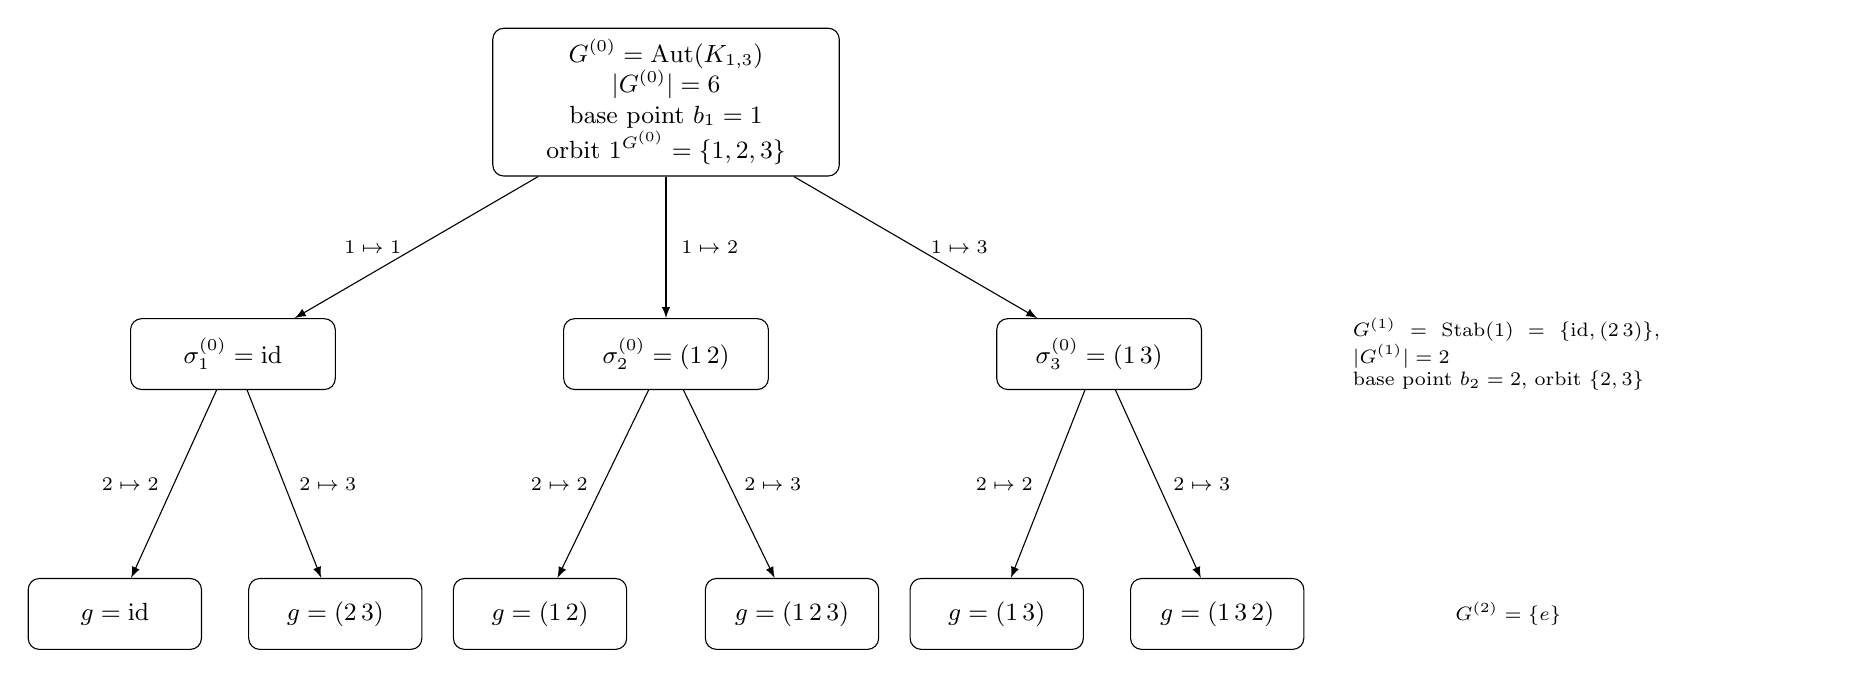
\begin{tikzpicture}[
  every node/.style={font=\small},
  level0/.style={draw, rounded corners, align=center, minimum width=4.4cm, minimum height=1.6cm, inner sep=4pt},
  level1/.style={draw, rounded corners, align=center, minimum width=2.6cm, minimum height=0.9cm, inner sep=3pt},
  leaf/.style={draw, rounded corners, align=center, minimum width=2.2cm, minimum height=0.9cm, inner sep=3pt},
  side/.style={align=left, font=\scriptsize, text width=4.6cm, anchor=west},
  >=latex
]

% --- Niveau 0 : G^{(0)} = Aut(K_{1,3}), |G^{(0)}|=6 ---
\node[level0] (root) at (0,7)
  {$G^{(0)} = \mathrm{Aut}(K_{1,3})$\\ $|G^{(0)}|=6$\\
   base point $b_1=1$\\ orbit $1^{G^{(0)}}=\{1,2,3\}$};

% --- Niveau 1 : trois cosets de G^{(1)} ---
\node[level1] (A) at (-5.5,3.8) {$\sigma^{(0)}_1=\mathrm{id}$};
\node[level1] (B) at (0,3.8)    {$\sigma^{(0)}_2=(1\,2)$};
\node[level1] (C) at (5.5,3.8)  {$\sigma^{(0)}_3=(1\,3)$};

\draw[->] (root) -- (A) node[pos=0.5, left=2pt]  {\scriptsize $1\mapsto1$};
\draw[->] (root) -- (B) node[pos=0.5, right=2pt] {\scriptsize $1\mapsto2$};
\draw[->] (root) -- (C) node[pos=0.5, right=2pt] {\scriptsize $1\mapsto3$};


\node[side] at (8.6,3.8)
{$G^{(1)}=\mathrm{Stab}(1)=\{\mathrm{id},(2\,3)\}$, $|G^{(1)}|=2$\\
 base point $b_2=2$, orbit $\{2,3\}$};

% --- Niveau 2 : les feuilles ---
\node[leaf] (A1) at (-7,0.5)   {$g=\mathrm{id}$};
\node[leaf] (A2) at (-4.2,0.5) {$g=(2\,3)$};
\node[leaf] (B1) at (-1.6,0.5) {$g=(1\,2)$};
\node[leaf] (B2) at (1.6,0.5)  {$g=(1\,2\,3)$};
\node[leaf] (C1) at (4.2,0.5)  {$g=(1\,3)$};
\node[leaf] (C2) at (7,0.5)    {$g=(1\,3\,2)$};

\draw[->] (A) -- (A1) node[pos=0.5, left=2pt]  {\scriptsize $2\mapsto2$};
\draw[->] (A) -- (A2) node[pos=0.5, right=2pt] {\scriptsize $2\mapsto3$};
\draw[->] (B) -- (B1) node[pos=0.5, left=2pt]  {\scriptsize $2\mapsto2$};
\draw[->] (B) -- (B2) node[pos=0.5, right=2pt] {\scriptsize $2\mapsto3$};
\draw[->] (C) -- (C1) node[pos=0.5, left=2pt]  {\scriptsize $2\mapsto2$};
\draw[->] (C) -- (C2) node[pos=0.5, right=2pt] {\scriptsize $2\mapsto3$};

% --- étiquette de niveau, à droite, alignée avec la rangée des feuilles ---
\node[side] at (9.9,0.5) {$G^{(2)}=\{e\}$};

\end{tikzpicture}%
  }
  \caption{Tree associated with the BSGS of $\mathrm{Aut}(K_{1,3})$ with base $(b_1=1,b_2=2)$.}
\end{figure}

We observe that each edge at level $i$ carries a transversal element $\sigma_p^{(i)}$ for the
orbit of $b_{i+1}$ under $G^{(i)}$; a leaf is the element of $G$ obtained by
composing these labels along its root-to-leaf path. Since the successive
orbits have sizes $3$, $2$, $1$, the tree has $3 \times 2 \times 1 = 6$
leaves. This is exactly the elements of $\mathrm{Aut}(K_{1,3})$.


\subsubsection{Schreier-Sims for \Naut{}}

Let $G$ be the input graph and $\pi_0$ its initial partition. Unlike
the setting described above, where Schreier-Sims is applied to a group
given by a known generating set, the automorphism group
$\mathrm{Aut}(G,\pi_0)$ is not known in advance here: its generators
are discovered incrementally, one by one, over the course of the search.

\Naut{} performs a depth-first traversal of the search tree. Each leaf
$\sigma$ corresponds to a permutation $R(G,\pi_0,\sigma)$, obtained
by applying the refinement function along the individualisation sequence
$\sigma$. Whenever a newly reached leaf $\sigma'$ produces the same
invariant as the first leaf $\sigma_0$ reached by the search, the permutation
\[
g = R(G,\pi_0,\sigma')\,R(G,\pi_0,\sigma_0){^{-1}}
\]
is an automorphism of $G$, and is added to the currently known
automorphism group.

These discovered automorphisms are the generators from which the group
structure is built. The automorphism $g$ is then sifted through the
existing stabiliser chain, correcting its action on each base point
successively. It is either absorbed by an existing level, in which case
it provides no new information, or it is identified as a new strong
generator and enriches the chain.

Each automorphism discovered at a leaf is propagated to the ancestor
nodes for which it remains relevant. The accumulated group information
is then used when selecting the next vertex to individualise. Once a
target cell has been chosen, its vertices are partitioned into orbits
under the currently known automorphism group. Two vertices belonging to
the same orbit necessarily lead to isomorphic subtrees, since they are
related by an automorphism already known to the algorithm. Consequently,
it is sufficient to explore a single representative of each orbit, while
all other vertices can be pruned without exploration.

This is a direct application of the pruning operation $\mathcal{P}_C$.

To get a concrete idea of what this looks like in code, here is a
simplified pseudo-code of the Schreier-Sims method for \Naut{}.

\noindent\fbox{%
  \parbox{\linewidth-2\fboxsep-2\fboxrule}{%
    \textit{Pseudo-code of Schreier-Sims method for \Naut{}} 

    \vspace{0.5em}
\begin{algorithmic}[1]
  \State\textbf{Data:} graph $G$, initial partition $\pi_0$, reference leaf $\sigma_0$, current base $B$
  \State\textbf{Result:} BSGS
  
  \For{each leaf $\sigma'$ reached by the depth-first search}
  \If{$\phi(G,\pi_0,\sigma') = \phi(G,\pi_0,\sigma_0)$} 
  \State$g \gets R(G,\pi_0,\sigma')\, R(G,\pi_0,\sigma_0){}^{-1}$ \Comment{candidate automorphism}
          \If{$g \neq \mathrm{id}$}
              \State\Call{InsertGenerator}{$g$, level $1$}
          \EndIf{}
      \EndIf{}
  \EndFor{}
  
  \Statex{}
  
  \Procedure{InsertGenerator}{$g$, level $i$}
      \If{$B$ has no point at level $i$}
          \State{} choose a new base point $b_i$ moved by $g$
      \EndIf{}
      \State{} add $g$ to the strong generators at level $i$
      \State\Call{GrowOrbit}{$i$} \Comment{updates the orbit and transversal at level $i$}
      \State\Call{Closestabiliser}{$i$} \Comment{Schreier generators, recurses if needed}
  \EndProcedure\end{algorithmic}
  }%
  }

 \newpage

  \subsubsection{Random Schreier method}

  The main difference between the classical Schreier-Sims algorithm seen previously and the Random Schreier method lies in the way the BSGS is constructed. Instead of deterministically maintaining an exact base and strong generating set from every newly discovered automorphism, the Random Schreier method adopts a probabilistic approach. It repeatedly generates random products of the automorphisms already known and inserts these permutations into the Schreier-Sims structure.
  
  This randomisation trades a deterministic guarantee for speed: the
  resulting approximation of the BSGS is correct with high probability
  rather than with certainty, in the Monte Carlo sense. Babai, Cooperman,
  Finkelstein, Luks and Seress showed that random products of the known
  generators emulate genuinely random group elements closely enough to
  yield a nearly optimal $O(n^3 \log^c n)$ membership
  test~\cite{babai1991fast}.
  
  The objective is not to compute the complete BSGS as early as possible, but rather to obtain a sufficiently rich approximation of the subgroup generated by the discovered automorphisms. This approximation often provides accurate orbit information much earlier during the search, allowing the $\mathcal{P}_C$ pruning strategy to eliminate redundant branches sooner. Consequently, the search tree may become significantly smaller.
  
  Since the method relies on randomisation, its effectiveness depends on the input graph. For many highly symmetric graphs, it substantially improves the pruning process. However, for graphs with few automorphisms, the additional computations required to generate and process random group elements may outweigh the benefits. For this reason, the Random Schreier method is implemented as an optional feature in \Naut{}.


  \newpage
  \subsubsection{Pruned search tree construction}

  To illustrate how the $\mathcal{P}_C$ pruning strategy operates in practice, we return to our search tree for $K_{1,3}$ (c.f.~\cref{fig:nauty-tree-k13}) and apply the $\mathcal{P}_C$ pruning strategy.
  
  \begin{figure}[htbp]
      \centering
      \resizebox{\linewidth}{!}{%
          % Encircle a target cell inline.
\newcommand{\tc}[2][black]{%
\tikz[baseline= (c.base)]{
\node[
    draw=#1,
    text=#1,
    ellipse,
    inner sep=1.5pt,
    outer sep=0pt,
    line width=0.4pt
] (c) {#2};
}%
}

\tikzset{
  stepmark/.style={
    circle, draw=black, fill=white,
    inner sep=0pt, minimum size=4.2mm,
    font=\tiny\bfseries, line width=0.4pt
  }
}



\newcommand{\ktgraph}[4][black]{%
\begin{tikzpicture}[
    scale=0.42,
    every node/.style={
        circle,
        draw=#1,
        text=#1,
        inner sep=0pt,
        minimum size=6mm,
        font=\tiny,
        line width=0.5pt
    }
]

\node (g0) at (0,0) {0};

\node[#2] (g1) at (-1.15,1.15) {1};
\node[#3] (g2) at (0,1.55) {2};
\node[#4] (g3) at (1.15,1.15) {3};

\draw[#1] (g0)--(g1);
\draw[#1] (g0)--(g2);
\draw[#1] (g0)--(g3);

\end{tikzpicture}%
}






\begin{tikzpicture}[
    every node/.style={font=\small}
]


% ---------- Initial partition ----------
\node[anchor=north,align=center] (init) at (8.75,14)
{
\ktgraph{}{}{}\\[2pt]
$\pi_0 = [\,0,1,2,3\,]$
};


% ---------- First refinement ----------
\node[anchor=north,align=center] (root) at (8.75,10)
{
\ktgraph{}{}{}\\[2pt]
$[\,0 \mid \tc{1,2,3}\,]$
};

\draw[
->,
line width=0.5pt
]
(init.south) --
(root.north)
node[midway,right]
{\scriptsize First Refinement};


% ---------- Level 1 ----------
\node[anchor=north,align=center] (A) at (1.75,6)
{
\ktgraph{double}{}{}\\[2pt]
$[\,0 \mid 1 \mid \tc{2,3}\,]$
};

\node[anchor=north,align=center] (B) at (8.75,6)
{
\ktgraph{}{double}{}\\[2pt]
$[\,0 \mid 2 \mid \tc{1,3}\,]$
};

\node[anchor=north,align=center,draw=gray,dashed,rounded corners,inner sep=4pt] (C) at (15.75,6)
{
\ktgraph[gray]{}{}{double}\\[2pt]
{\color{gray}$[\,0 \mid 3 \mid \tc[gray]{1,2}\,]$}\\[4pt]
{\scriptsize\itshape\color{gray} Pruned by automorphism $(2\ 3)$}
};


% ---------- Leaves ----------
\node[anchor=north,align=center] (L1) at (0,1.2)
{
\ktgraph{double}{double}{}\\[2pt]
$[\,0 \mid 1 \mid 2 \mid 3\,]$
};

\node[anchor=north,align=center] (L2) at (3.5,1.2)
{
\ktgraph{double}{}{double}\\[2pt]
$[\,0 \mid 1 \mid 3 \mid 2\,]$
};

\node[anchor=north,align=center] (L3) at (7,1.2)
{
\ktgraph{}{double}{ }\\[2pt]
$[\,0 \mid 2 \mid 1 \mid 3\,]$
};

\node[anchor=north,align=center,draw=gray,dashed,rounded corners,inner sep=4pt] (L4) at (10.5,1.2)
{
\ktgraph[gray]{}{double}{double}\\[2pt]
{\color{gray}$[\,0 \mid 2 \mid 3 \mid 1\,]$}\\[4pt]
{\scriptsize\itshape\color{gray} Pruned by automorphism $(1\ 3)$}
};

\node[anchor=north,align=center,draw=gray,dashed,rounded corners,inner sep=4pt] (L5) at (14,1.2)
{
\ktgraph[gray]{}{}{double}\\[2pt]
{\color{gray}$[\,0 \mid 3 \mid 1 \mid 2\,]$}\\[4pt]
{\scriptsize\itshape\color{gray} Not generated}
};

\node[anchor=north,align=center,draw=gray,dashed,rounded corners,inner sep=4pt] (L6) at (17.5,1.2)
{
\ktgraph[gray]{}{double}{double}\\[2pt]
{\color{gray}$[\,0 \mid 3 \mid 2 \mid 1\,]$}\\[4pt]
{\scriptsize\itshape\color{gray} Not generated}
};


% ---------- Target cell labels ----------
\draw[dashed,->]
(root.east) -- ++(1.2,0)
node[right]{\scriptsize Target cell};

\draw[dashed,->]
(A.east) -- ++(1.1,0)
node[right]{\scriptsize Target cell};

\draw[dashed,->]
(B.east) -- ++(1.1,0)
node[right]{\scriptsize Target cell};

\draw[dashed,gray,->]
(C.east) -- ++(1.1,0)
node[right]{\scriptsize\color{gray} Target cell};


% ---------- Edges ----------
\draw (root.south) -- (A.north)
node[midway,above left] {$1$};

\draw (root.south) -- (B.north)
node[midway,right] {$2$};

\draw[dashed,gray] (root.south) -- (C.north)
node[midway,above right,gray] {$3$};


\draw (A.south) -- (L1.north)
node[midway,left] {$2$};

\draw (A.south) -- (L2.north)
node[midway,right] {$3$};


\draw (B.south) -- (L3.north)
node[midway,left] {$1$};

\draw[dashed,gray] (B.south) -- (L4.north)
node[midway,right,gray] {$3$};


\draw[dashed,gray] (C.south) -- (L5.north)
node[midway,left,gray] {$1$};

\draw[dashed,gray] (C.south) -- (L6.north)
node[midway,right,gray] {$2$};


% ---------- Step markers ----------
\node[stepmark] at ($(init.north west)+(-0.3,0.3)$) {1};
\node[stepmark] at ($(L1.north west)+(-0.3,0.3)$) {2};
\node[stepmark] at ($(L2.north east)+(-0.3,0.3)$) {3};
\node[stepmark] at ($(B.north east)+(-0.3,0.3)$) {4};
\node[stepmark] at ($(L3.north west)+(0.3,0.3)$) {5};
\node[stepmark] at ($(L4.north east)+(-1,0.4)$) {6};
\node[stepmark] at ($(C.north east)+(-1,0.4)$) {7};




\end{tikzpicture}
      }
      \caption{Search tree for $K_{1,3}$ with the $\mathcal{P}_C$ pruning strategy applied.}\label{fig:nauty-tree-k13-prunned}
  \end{figure}
  
  To better understand how this strategy works, we will walk through the construction of the pruned search tree step by step, highlighting the discovered automorphisms and the branches that are pruned.
  
  \begin{itemize}
    \item[\textcircled{1}] We start from the original graph.
    \item[\textcircled{2}] The first leaf reached, obtained by individualising $1$, then $2$, then $3$, is taken as the reference leaf against which every subsequent leaf is compared.
    \item[\textcircled{3}] Comparing the second leaf to the reference leaf yields the automorphism $(2\ 3)$.
    \item[\textcircled{4}] When vertex $2$ is individualised, none of the automorphisms found so far allow pruning any of its children. The target cell $\{1,3\}$ is therefore kept in full.
    \item[\textcircled{5}] Individualising $1$ next yields a leaf whose comparison with the reference leaf gives the automorphism $(1\ 2)$. Combined with $(2\ 3)$ found earlier, this closes the automorphism group to $S_3$, which in particular contains $(1\ 3)$.
    \item[\textcircled{6}] This new automorphism is then used to prune the remaining leaf of that branch.
    \item[\textcircled{7}] Likewise, $(2\ 3)$ shows that individualising vertex $3$ first is equivalent to individualising vertex $2$ first. The corresponding branch is therefore pruned entirely, without ever being explored.
  \end{itemize}

\subsection{Final search tree construction}

We can put in practice our different pruning strategies on our search tree. \Naut{} will generate its tree in depth-first order. The lexicographically least leaf $\sigma_1$ is kept and if the canonical labelling is sought (rather than just the automorphism group), the leaf $\sigma^*$ with the greatest invariant discovered so far is also kept. A non-discrete node $\sigma$ is pruned if neither $\phi(G,\pi_0, \sigma) = \phi(G,\pi_0, {[\sigma_1]}_{|\sigma|})$ or $\phi(G,\pi_0, \sigma) \geq\phi(G,\pi_0, {[\sigma^*]}_{|\sigma|})$. Such operations correspond to $\mathcal{P}_A (\sigma^*, \sigma)$ and $\mathcal{P}_B (\sigma_1, \sigma)$. We can therefore conclude that only a subset of the tree will be generated, and that the generated leaves are those that may be ``better'' than the leaves already discovered.



\noindent\fbox{%
  \parbox{\linewidth-2\fboxsep-2\fboxrule}{%
    \textit{Pseudo-code of canonical labelling} 

    \vspace{0.5em}

    \begin{algorithmic}[1]
      \State\textbf{Data:} A graph $G = (V, E)$
      \State\textbf{Result:} The canonical form of $G$

      \vspace{0.4em}

      \State$\pi \leftarrow (\{0, 1, \dots, |V|-1\})$
      \State$\pi  \leftarrow F(G, \pi , \text{a list of all the cell of } 
      \pi)$ 
      \State$\pi ^* \leftarrow \pi$ \Comment{$\pi^*$ the best partition}
      \State$\pi_1 \leftarrow () $ \Comment{$\pi_1$ the partition of first leaf}
      \State$\sigma \leftarrow ()$, \quad $\sigma^* \leftarrow ()$ \Comment{current and best vertex sequences}

      \vspace{0.4em}

      \Procedure{NAUTY}{$G,\, \pi $}
        \If{$\pi$ is discrete}
          \If{$\pi^*$ is not discrete} \Comment{no leaf found yet}
            \State$\pi^*\leftarrow\pi$,\ $\sigma^*\leftarrow\sigma$,\ $\pi_1\leftarrow\pi$
            \State{}BSGS $\leftarrow$ Base ($\sigma$) \Comment{initialise Base}
          \ElsIf{$\phi(G,\pi,\sigma) > \phi(G,\pi^*,\sigma^*)$}
            \State$\pi^*\leftarrow\pi$,\ $\sigma^*\leftarrow\sigma$ \Comment{better leaf found}
          \EndIf{}
          \State\Return{}
        \EndIf{}
        \If{$\pi^*$ is discrete \textbf{and} $\phi(G,\pi,\sigma) < \phi(G,\pi^*,\sigma^*)$ \textbf{and} $\phi(G,\pi,\sigma)\neq\phi(G,\pi_1,\sigma_1)$}
          \State\Return\Comment{Pruning $\mathcal{P}_A+\mathcal{P}_B$: cannot beat $\pi^*$, nor tie $\pi_1$}
        \EndIf{}
        \State$\text{Cell} \leftarrow T(G,\pi,\sigma)$
        \State$R \leftarrow$ orbit representatives of $\text{Cell}$ \Comment{Pruning $\mathcal{P}_C$}
        \For{each $\nu \in R$}
          \State{$\pi _\nu \leftarrow I(\pi , \nu)$}
          \State{$\pi _\nu \leftarrow F(G,\, \pi _\nu,\,\{\nu\})$}
          \State{Append $\nu$ to $\sigma$}
          \State\Call{NAUTY}{$G,\, \pi _\nu$}
          \State{Remove last entry from $\sigma$}
        \EndFor\EndProcedure\vspace{0.3em}

      \State$g \leftarrow$ canonical vertex ordering induced by $\pi^*$
      \State\Return{$G^g$} \Comment{Apply g to $G$ to get the canonical form}

    \end{algorithmic}
  }%
}




